%==============================================================================
% Research-mode example for the OSU / Soundbendor beamer style.
% Every style decision lives in sty/osu.sty; this file is content only.
% Build:  latexmk -pdf research.tex   (biber runs automatically)
%==============================================================================
\documentclass[10pt,aspectratio=169,xcolor=table]{beamer}
\usepackage[campus=corvallis, mode=research]{sty/osu}

\usepackage[style=ieee]{biblatex}
\addbibresource{refs.bib}

\title{Purr-ceptual Evaluation}
\subtitle{Detecting Feline Disapproval of Human Playlists with Very Deep Learning}
\author{A. Grad Student \and P. I. Advisor}
\institute{Soundbendor Lab \textperiodcentered\ Oregon State University}
\date{\today}

\begin{document}
\maketitle

%------------------------------------------------------------------------------
\begin{frame}{Outline}
  \tableofcontents
\end{frame}

%==============================================================================
\section{Motivation}
%==============================================================================

\begin{frame}{The Problem}
  \begin{columns}[T]
    \column{0.55\textwidth}
      \begin{itemize}
        \item Humans play music near cats \alert{constantly}
        \item Cats have opinions \alert{constantly}
        \item Nobody has asked them
          \begin{itemize}
            \item Mostly because they don't fill out surveys
            \item Partly because they knock the clipboard off the table
          \end{itemize}
      \end{itemize}
      \medskip
      \begin{rq}
        Can a model predict when a cat leaves the room \emph{because of the music}?
      \end{rq}
      \begin{rq}[The Jazz Question]
        Is it always the jazz?
      \end{rq}
    \column{0.4\textwidth}
      \bignumber{73\%}{of cats left the room within 30\,s of the
        first saxophone solo\footnotemark}
  \end{columns}
  \footnotetext{The other 27\% were asleep, which we count as a strong negative review.}
\end{frame}

\begin{frame}{Prior Work}
  \begin{itemize}
    \item Attention mechanisms for cats \cite{whiskers2024attention}
    \item Mel-spectrograms, but for meows \cite{mittens2023meowl}
    \item Large-scale napping datasets \cite{loaf2025, whiskers2024attention}
    \item The observer problem: the cat changes state when you check on it
          \cite{schrodinger1935}
  \end{itemize}
  \bigskip
  \begin{bigquote}[Reviewer 2]
    The authors should also evaluate on dogs.
  \end{bigquote}
  \slidecite{All references are fictional, except one, sort of.}
\end{frame}

%==============================================================================
\section{Method}
%==============================================================================

\begin{frame}{Pipeline}
  \centering
  \begin{tikzpicture}[
      node distance=6mm and 9mm, every node/.append style={minimum width=22mm}]
    \node[osunode=stratosphere] (audio) {Playlist\\audio};
    \node[osunode=pinestand, right=of audio] (mel) {Mel\\spectrogram};
    \node[osunode=luminance, right=of mel] (net) {CatNet\\(152 layers)};
    \node[osunode=beaver, right=of net] (out) {P(cat\\leaves room)};
    \node[osunode=highdesert, below=of mel] (cam) {Hallway\\camera};
    \draw[osuarrow] (audio) -- (mel);
    \draw[osuarrow] (mel) -- (net);
    \draw[osuarrow] (net) -- (out);
    \draw[osuarrow] (cam) -| node[pos=0.25, below, font=\scriptsize]{labels} (net);
  \end{tikzpicture}
  \bigskip

  \begin{hypothesis}
    Feline disapproval grows linearly with tempo (BPM).
  \end{hypothesis}
  \begin{hypothesis}<2->
    \sout<3->{Cats are a uniform population.}
    \only<3>{\hfill\stress{Rejected by Professor Biscuits, our only participant.}}
  \end{hypothesis}
\end{frame}

\begin{frame}{Objective}
  We pick the playlist that the cat dislikes least:
  \[
    \hat{\pi} \;=\; \argmin_{\pi \in \Pi}\;
      \E_{t \sim \pi}\!\left[\, P\left(\text{leave} \given \mathbf{x}_t\right) \right]
      \;+\; \lambda \norm{\theta}_2^2
  \]
  where $\mathbf{x}_t \in \R^{128 \times T}$ is the mel spectrogram of track
  $t$ and $\lambda$ is the \keyword{treat-based regularizer}.
  \medskip

  \begin{aside}[Notation]
    \var{leave} is a binary event. Cats returning to the room to stare at
    you is modeled separately as \mat{$\mathbf{W}_{\text{judge}}$}.
  \end{aside}
\end{frame}

\begin{frame}[fragile]{Training Procedure}
  \begin{columns}[T]
    \column{0.55\textwidth}
    \begin{algorithm}[H]
      \caption{CatNet training}
      \Input{playlist $\Pi$, cat $c$, treats $k$}
      \Output{model parameters $\theta$}
      \BlankLine
      \SetKwFunction{FTrain}{Train}
      \Fn{\FTrain{$\Pi, c, k$}}{
        \ForEach{track $t \in \Pi$}{
          play $t$ \tcp*{at a respectful volume}
          \eIf{$c$ leaves the room}{
            $y_t \gets 1$\;
          }{
            $y_t \gets 0$\;
            $k \gets k - 1$ \tcp*{bribery}
          }
        }
        $\theta \gets \argmin_\theta \mathcal{L}(\theta; y)$\;
        \KwRet{$\theta$}\;
      }
    \end{algorithm}
    \column{0.4\textwidth}
      \begin{lstlisting}[style=numbered]
def loss(y_hat, y):
    # standard BCE, but
    # the cat judges you
    bce = F.binary_cross_entropy(
        y_hat, y)
    return bce * JUDGEMENT
\end{lstlisting}
      \todo{is JUDGEMENT a hyperparameter?}
  \end{columns}
\end{frame}

%==============================================================================
\section{Results}
%==============================================================================

\begin{frame}{Disapproval by Genre}
  \begin{columns}[c]
    \column{0.58\textwidth}
    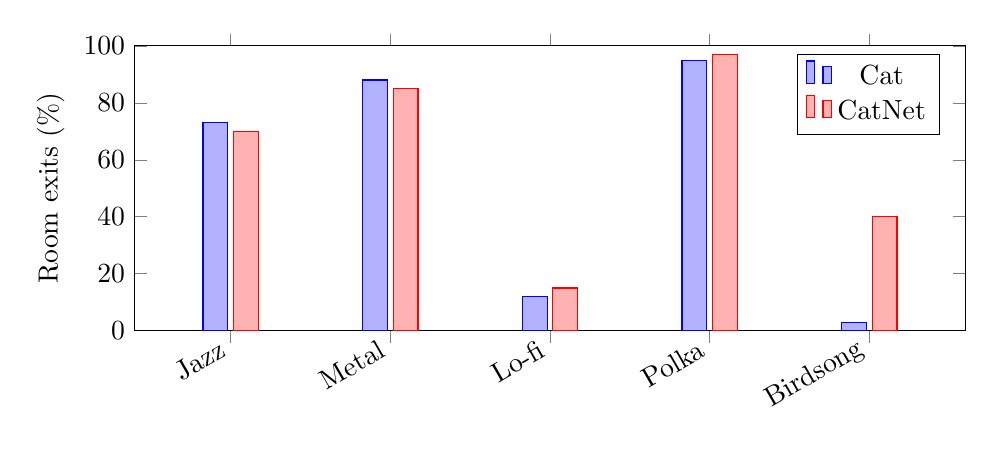
\begin{tikzpicture}
      \begin{axis}[
          ybar, bar width=9pt, width=\linewidth, height=5.2cm,
          ymin=0, ymax=100, ylabel={Room exits (\%)},
          symbolic x coords={Jazz, Metal, Lo-fi, Polka, Birdsong},
          xtick=data, x tick label style={rotate=30, anchor=east},
          legend pos=north east, enlarge x limits=0.15]
        \addplot coordinates {(Jazz,73) (Metal,88) (Lo-fi,12) (Polka,95) (Birdsong,3)};
        \addplot coordinates {(Jazz,70) (Metal,85) (Lo-fi,15) (Polka,97) (Birdsong,40)};
        \legend{Cat, CatNet}
      \end{axis}
    \end{tikzpicture}
    \column{0.38\textwidth}
      \begin{finding}
        CatNet agrees with the cat on everything except \stress{birdsong}.
        The cat walks toward the window. CatNet does not have legs.
      \end{finding}
      \begin{limitation}
        $n = 1$ cat.
      \end{limitation}
  \end{columns}
\end{frame}

\begin{frame}{Comparison With Baselines}
  \centering
  \rowcolors{2}{beaver!8}{white}
  \begin{tabular}{lrrr}
    \toprule
    \textbf{Model} & \textbf{Accuracy} & \textbf{Params} & \textbf{Treats used} \\
    \midrule
    Random guess         & 50.0 & 0     & 0 \\
    Always ``leaves''    & 61.2 & 0     & 0 \\
    Graduate student     & 64.8 & $\sim$86\,B & 312 \\
    CatNet (ours)        & \textbf{91.4} & 152\,M & 2{,}048 \\
    CatNet + nap prior   & \textbf{93.0} & 152\,M & \textbf{4{,}096} \\
    \bottomrule
  \end{tabular}
  \bigskip

  \begin{itemize}
    \item Graduate students underperform because they also leave the room for jazz.
  \end{itemize}
\end{frame}

{\metroset{block=transparent}
\begin{frame}{Ablation}
  \begin{columns}[T]
    \column{0.48\textwidth}
      \begin{exampleblock}{What helped}
        \begin{itemize}
          \item More layers
          \item More treats
          \item Closing the door
        \end{itemize}
      \end{exampleblock}
    \column{0.48\textwidth}
      \begin{alertblock}{What did not}
        \begin{itemize}
          \item Explaining the research to the cat
          \item Playing the cat's own meows back to it
        \end{itemize}
      \end{alertblock}
  \end{columns}
\end{frame}
}

%==============================================================================
\section{Conclusion}
%==============================================================================

\begin{frame}{Contributions}
  \begin{contribution}
    The first dataset of feline playlist reactions: \textbf{1 cat},
    \textbf{4{,}000 tracks}, \textbf{0 consent forms}.
  \end{contribution}
  \begin{contribution}[Open Source]
    Code and model weights at the link below. The cat's weight is private.
  \end{contribution}
  \begin{futurework}
    Dogs (per Reviewer 2). Early results: dogs like everything.
  \end{futurework}
  \vfill
  \begin{columns}[c]
    \column{0.2\textwidth}\qrlink[1.6cm]{https://soundbendor.org}
    \column{0.75\textwidth}\small Paper, code, and an apology to Professor Biscuits:
      \url{https://soundbendor.org}
  \end{columns}
\end{frame}

\begin{frame}[standout]
  Questions?\\[0.5em]
  {\normalsize (Please do not ask about the dog study.)}
\end{frame}

%==============================================================================
\appendix
%==============================================================================

\begin{frame}{Backup: Full Confusion Matrix}
  \centering
  \begin{confusionmatrix}{Cat (actual)}{CatNet (predicted)}{stays, leaves, glares}
    \cmrow{stays}{412, 31, 7}
    \cmrow{leaves}{38, 519, 2}
    \cmrow{glares}{11, 4, 976}
  \end{confusionmatrix}
  \bigskip

  Correct predictions are on the shaded diagonal. ``Glares'' is the most common
  class and, according to the cat, the default.\par\medskip
  {\small Appendix slides are not counted in the frame total.}
\end{frame}

\begin{frame}[allowframebreaks]{References}
  \printbibliography[heading=none]
\end{frame}

\end{document}
